\documentclass[11pt,twoside,a4paper]{article} % scrartcl

\usepackage{amsmath}
\usepackage[hidelinks]{hyperref}
\usepackage[utf8]{inputenc}
\usepackage{mdframed}
\usepackage{qtree}
\usepackage{tikz}
\usetikzlibrary{arrows,shapes,calc,decorations.pathreplacing}

\newcommand{\nonterm}[1]{$\left<#1\right>$}
\newcommand{\alt}[0]{$|$}

\begin{document}
\title{Introduction to Lambda Calculus}
%\subtitle{notes}
\author{Maciek Makowski}
\maketitle

\section{Motivation}

Software is pervasive in the modern world and has influence over many aspects 
of our lives. In some cases, such as avionics or medical equipment control, 
human life depends on the correctness of software. Yet, high profile cases of 
bugs\footnote{Infamous historical examples include Mars Climate 
Orbiter's inconsistent usage of units of measurement\cite{mco} and Therac-25 
radiation therapy overdoses\cite{therac25}. Recent faults such as
security-related Apple goto fail\cite{cve141266} and OpenSSL Heartbleed
bug\cite{cve140160},
while not life-threatening, had wide-ranging implications for the security of
e-commerce and privacy of internet users.} do not inspire confidence in the 
state of software engineering. The "software crisis" is a phenomenon recognised 
by practitioners of the field. A number of ways to address the reliability issue 
has been proposed, from reliance on programmer's 
discipline\cite{cleancode}\cite{securecoding}, through tools that
analyse programs written in popular languages for suspicious 
patterns\cite{raf04}, to languages that restrict valid programs to ones whose 
properties can be formally proven. The latter approach relies on a body of 
theoretical knowledge that can appear intimidating. It turns out, 
however, that much of the required insight is built on systematic extensions of 
a very simple formal system -- the lambda calculus. Familiarity with the 
fundamentals of lambda calculus is a prerequisite for proficiency with modern 
software engineering tools. These notes aim to introduce lambda calculus in a 
very informal manner. The only background assumed is that of general programming 
experience.

\section{Syntax}

Given a set of variables $X$, terms of lambda calculus are generated by the 
following grammar:
\begin{tabbing}
\nonterm{term} \= ::=  \= $x$~~~~~~~~~~~~~~~~~~~~~~~~~~~~ \= (variable)    \\
               \> \alt \> ($\lambda x.$\nonterm{term})    \> (abstraction) \\
               \> \alt \> (\nonterm{term} \nonterm{term}) \> (application) \\
\end{tabbing}
where $x\in X$. Notational convention is that application binds to the left, the 
full-stop can be treated as an opening parenthesis that extends until the end of 
the sub-term and redundant parentheses are omitted. Examples of lambda terms 
as they are typically written, together with ASTs they represent:
\begin{tabbing}
$v_1$~~~~~~~~~~~~~~~~~~~~~~~~~~~~~~~~~~~~~~ \= \Tree [.{var $v_1$} ]           \\
\noindent\rule{12.5cm}{0.4pt}                                                  \\
$x\ y\ z$                                   \> \Tree [.app [.app {var $x$} 
{var $y$} ] {var $z$} ]                                                        \\
\noindent\rule{12.5cm}{0.4pt}                                                  \\
$(\lambda a.\lambda b.a)\ c\ (\lambda b.b)$ \> \Tree [.app [.app [.{abs $a$} 
[.{abs $b$} {var $a$} ] ] {var $c$} ] [.{abs $b$} {var $b$} ] ]                \\
\end{tabbing}
Within a term, occurrences of variables that are not bound by enclosing abstraction
-- i.e. where the variable name does not appear in any abs node on the path to the 
root of the AST -- are called \emph{free}. In the examples below free
occurrences are underlined:
\begin{itemize}
\item $\lambda x.\underline{y}$
\item $(\lambda a.\lambda \underline{b}.a)\ \underline{c}\ (\lambda b.b)$
\end{itemize}
Note that the same variable name might have both bound and free occurrences
within a term, as in the second example. Terms with no free occurrences are known 
as \emph{closed terms}, or \emph{combinators}.

\paragraph{Summary:} we have defined what lambda terms look like. The grammar 
has three productions -- variable, abstraction and application -- and generates 
abstract syntax trees.

\section{Rewriting Rules}

Lambda terms are not of much use without some operations that can be performed
on them. Two\footnote{The third frequently applied operation is introduction/removal 
of abstraction ($\eta$-conversion): $\lambda x.M\,x\longleftrightarrow_\eta M$ for 
any term $M$. We will not require it in this presentation of lambda calculus.} 
operations we will use going forward are presented below.

\subsection{Renaming of bound variables}

Intuitively, $\lambda x.x$ is similar to $\lambda y.y$ -- the "shape" of these
two terms is the same, they differ only in the choice of variable used. In 
practice we will often want to identify terms of the same structure. 
This intuitive similarity is captured by an operation called 
\emph{$\alpha$-conversion} that consistently renames variables. While the
operation appears trivial, there are subtleties around bound vs. free
variables -- for instance, nested abstractions can use the same variable name
-- but these difficulties manifest themselves mostly in the
implementation\footnote{For that reason a convenient way to represent 
lambda terms when implementing evaluation is positional (de Bruijn) encoding
which replaces variable names with numerical index of the lambda that binds given 
variable occurrence. For example, de Bruijn representation of 
$\lambda a.\lambda b.a\ b\ c$  would be $\lambda.\lambda.1\ 0\ 2$ under naming 
context $\{c\mapsto 2\}$.  The naming context is required to map free variables 
to indices.}, so we will not worry about them in this presentation. The intuition 
about variable renaming is correct in most cases we are interested in. In 
particular, we can assume that all the variables in the terms we are working 
with have been chosen so that they are distinct. It is always possible to 
$\alpha$-convert any term so that this is true.
\paragraph{Example:} $(\lambda x.x\,y)\ (\lambda x.x)\longleftrightarrow_\alpha(\lambda
a.a\,y)\ (\lambda b.b)$

\subsection{Removal of abstraction under application}

TODO: \emph{$\beta$-reduction}

\paragraph{Example:} $(\lambda x.x\,y)\ (\lambda z.z)\longrightarrow_\beta
(\lambda z.z)\ y\longrightarrow_\beta y$

In the first reduction, $\lambda x.$ is eliminated by substituting $\lambda z.z$ 
for $x$, in the second, $\lambda z.$ is eliminated by substituting $y$ for $z$.

This is the key operation of lambda calculus, as it represents a
\emph{computation}. It allows us to view a lambda term as a program that can be
evaluated to a final value (i.e. a term that cannot be further reduced). That
final value is called a \emph{normal form} of a term.

An application that can be $\beta$-reduced is called a \emph{redex}. There can
be multiple redexes in a given term:

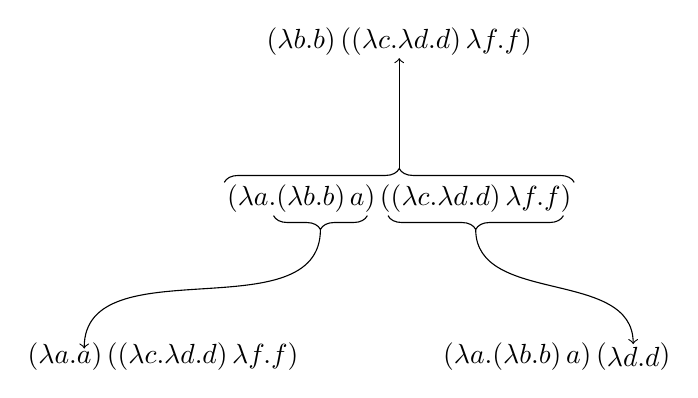
\begin{tikzpicture}[every node/.style={inner sep=0,outer sep=1}]
    \node[matrix](s1) at (3,0) {
        \node     {$(\lambda a.$}; &
        \node(s2) {$(\lambda b.b)\,a$}; &
        \node     {$)\,($}; &
        \node(s3) {$(\lambda c.\lambda d.d)\,\lambda f.f$}; &
        \node     {$)$}; \\
    };
    \node(d1) at (3,2) {$(\lambda b.b)\,((\lambda c.\lambda d.d)\,\lambda f.f)$};
    \node[matrix] at (0,-2){
        \node                   {$(\lambda a.$}; &
        \node(d2) at (0, -0.01) {$a$}; &
        \node                   {$)\,((\lambda c.\lambda d.d)\,\lambda f.f)$}; \\
    };
    \node[matrix] at (5,-2){
        \node     {$(\lambda a.(\lambda b.b)\,a)\,($}; &
        \node(d3) {$\lambda d.d$}; &
        \node     {$)$}; \\
    };
    \draw[decorate,decoration={brace,amplitude=5pt}]
    (s1.north west)--(s1.north east);
    \draw[->] ($(s1.north)+(0,5pt)$) to node[right,midway]{}(d1);
    \draw[decorate,decoration={brace,mirror,amplitude=5pt}]
    (s2.south west)--(s2.south east);
    \draw[->] ($(s2.south)+(0,-5pt)$) to [out=-90,in=90] node{}(d2);
    \draw[decorate,decoration={brace,mirror,amplitude=5pt}]
    (s3.south west)--(s3.south east);
    \draw[->] ($(s3.south)+(0,-5pt)$) to [out=-90,in=90] node{}(d3);
\end{tikzpicture}

The choice of the redex to be reduced next is up to us. Prescribing which redex
should be chosen gives rise to a reduction strategy. For example:
\begin{itemize}
\item TODO: call-by-name
\item TODO: call-by-value
\end{itemize}

\paragraph{Summary:} lambda-terms can be syntactically transformed according to 
two rules: $\alpha$-conversion, which renames the variables, and $\beta$-reduction,
which "applies" one term to another.

\section{Programming}

We claimed that a lambda term can be treated as a computer program. To substantiate 
this, let us see how familiar elements of programming languages can be represented 
in lambda calculus.

\subsection{Conditionals}

TODO

\subsection{Numbers}

\begin{align*}
0 &= \lambda s.\lambda z.z \\
1 &= \lambda s.\lambda z.s\,z \\
2 &= \lambda s.\lambda z.s\,(s\,z) \\
3 &= \lambda s.\lambda z.s\,(s\,(s\,z)) \\
\end{align*}
\begin{mdframed}
In general, $n = \lambda s.\lambda z\underbrace{s\,(\dots s\,(s}_n\,z)\dots)$.
\end{mdframed}

TODO\footnote{Seeing how Peano arithmetic can be defined in lambda calculus,
and drawing parallels with Zermelo-Fraenkel set-theoretical model of
natural numbers and the build-out of other mathematical constructions on this
basis, one could ask: can untyped lambda calculus be treated as a foundational
theory in which all known mathematical concepts can be stated? Alonso Church had 
that in mind when he conceived lambda calculus, but it was soon proven by his 
studens, Kleene and Rosser\cite{wkrp}, that in fact the calculus as we present it here is 
inconsistent, i.e. any proposition can be proven in it.}

\subsection{Loops}

TODO

\section{Model of Computation}

TODO

\section{Church-Rosser Theorem}

TODO

\section{Curry-Howard Correspondence}

TODO

\section{Further Reading}

A direct inspiration for this talk was the presentation of lambda calculus in
\cite{TAPL}. The book is very well written and builds a sophisticated type
system in easy to follow steps, starting from untyped lambda calculus. 

For a succinct but rigorous introduction to lambda calculus see \cite{bb00}.

TODO

\begin{thebibliography}{9}
\bibitem{TAPL} Benjamin C. Pierce, \emph{Types and Programming Languages},
\url{http://www.cis.upenn.edu/~bcpierce/tapl/}
\bibitem{su99} Morten Heine B. Sørensen, Paweł Urzyczyn, \emph{Lectures on the
Curry-Howard Isomorphism}, 
\url{http://citeseerx.ist.psu.edu/viewdoc/summary?doi=10.1.1.17.7385}
\bibitem{bb00} Henk Berendregt, Erik Barendsen, \emph{Introduction to Lambda
Calculus}, 
\url{http://www.cse.chalmers.se/research/group/logic/TypesSS05/Extra/geuvers.pdf}
\bibitem{grue97} Klaus Grue, \emph{Lambda calculus as a foundation of mathematics},
\url{http://www.diku.dk/~grue/papers/church/church.html}
\bibitem{mco} NASA, \emph{Mars Climate Orbiter Team Finds Likely Cause of Loss}, 
\url{http://www.jpl.nasa.gov/news/releases/99/mcoloss1.html}
\bibitem{therac25} Nancy Leveson, Clark S. Turner, 
\emph{An Investigation of the Therac-25 Accidents}
\url{http://courses.cs.vt.edu/cs3604/lib/Therac_25/Therac_1.html}
\bibitem{cve141266} \emph{CVE-2014-1266},
\url{http://cve.mitre.org/cgi-bin/cvename.cgi?name=CVE-2014-1266}
\bibitem{cve140160} \emph{CVE-2014-0160}, 
\url{https://cve.mitre.org/cgi-bin/cvename.cgi?name=CVE-2014-0160}
\bibitem{cleancode} Robert C. Martin, \emph{Clean Code}
\bibitem{securecoding} various authors, \emph{CERT C Coding Standard}, 
\url{https://www.securecoding.cert.org/confluence/pages/viewpage.action?pageId=524435}
\bibitem{raf04} Nick Rutar, Christian B. Almazan, Jeffrey S. Foster, \emph{A
Comparison of Bug Finding Tools for Java}, 
\url{http://www.cs.umd.edu/~jfoster/papers/issre04.pdf}
\bibitem{wkrp} Wikipedia, \emph{Kleene-Rosser paradox},
\url{https://en.wikipedia.org/wiki/Kleene-Rosser_paradox}
\end{thebibliography}

\end{document}
